%======================================================================
\section{AI-assisted workflow and verification}\label{app:ai}
%======================================================================

This paper was produced with substantial assistance from an AI system (Claude, Anthropic), working in a code-executing environment under the direction of the author. The author chose the questions and the overall direction, and is responsible for every statement. The AI system drafted proofs, wrote and ran the numerical experiments, searched the literature, and wrote the working documents from which this paper was assembled. We record here what was explored, which claims had to be corrected, and how each result was checked. A reader can then judge which parts rest on what kind of evidence.

\subsection{Origin of the project}
The project began as an audit of an earlier programme, a ``seven-island'' route map, aimed at proving the twin prime conjecture through two bridges.
\begin{itemize}
\item \emph{Bridge A:} an operator-theoretic scalar estimate.
\item \emph{Bridge B:} hitting a distinguished point in a profinite dynamical system.
\end{itemize}
The audit substituted Selberg-type parity counterfeits into both bridges. These are sequences that preserve all Type~I information but flip the parity of the number of prime factors. The result was that each bridge is equivalent to the twin prime asymptotic itself, not weaker:
\begin{itemize}
\item the parity-sensitive ``gate'' of Bridge~A is the twin residual;
\item the cylinder criterion of Bridge~B contains its own conclusion.
\end{itemize}
These negative findings will appear separately. They motivated the present question: where exactly does parity enter, and which methods can see it?

\subsection{Numerical exploration}
Every numerical claim in this paper comes from a script in the project repository. The scripts are listed in Table~\ref{tab:scripts}. All computations are exact integer computations (sieves, factorisations, counts), except the Lanczos eigenvalue estimates and the least-squares fits.

\begin{table}[h]
\centering
\small
\begin{tabular}{p{3.6cm}p{5.6cm}p{3.4cm}}
\toprule
script & purpose & range\\
\midrule
\texttt{check\_compiler.py} & $M$, $D_1^\flat,D_2^\flat,D_3^\flat$, the parity identity (residual exactly $0$), $\rho_3(X)$ & $x\le10^7$\\
\texttt{parity\_patterns.py} & the four parity patterns of almost-prime pairs & $x\le10^7$\\
\texttt{rough\_parity\_model.py}, \texttt{rough\_chowla.py} & parity coupling on rough pairs & $x\le10^7$\\
\texttt{l1\_test.py} & $(s,r')$ fit; artificial worlds violating coherence & $x=10^7$\\
\texttt{l4\_experiment.py} & Lanczos for the rough divisibility operator & $x=10^8$\\
\texttt{barrier\_check.py} & constants of Lemma~\ref{lem:sieve-inputs}; $|\mathcal K|/(2E_R)$ & $x=10^7$\\
\texttt{cutoff\_ratio.py} & Table of Section~\ref{sec:coupling} & $N\le10^9$\\
\texttt{amplification.py} & search for dilation-closed weights with large parity imbalance & $x\le10^7$\\
\texttt{entropy\_test.py} & entropy budget, mutual information and decoupling, twin vs Chowla (Remark~\ref{rem:entropy-ceiling}) & $x\le10^8$\\
\texttt{bilinear\_probe.py} & $\mu(p+2)$ on all vs rough shifted values; FI Type~II sums (Remark~\ref{rem:lww-ceiling}) & $x\le10^8$\\
\texttt{pellet\_check.py} & Pellet's formula over $\mathbb F_3,\mathbb F_5$, by smallest factor degree (Section~\ref{sec:explored}) & $\deg\le7$\\
\texttt{parity\_lp.py} & multi-pattern parity linear program, H3 (Section~\ref{sec:explored}) & $\le966$ variables\\
\texttt{h6\_digits.py} & $\lambda$ vs function-field M\"obius of the base-$p$ digit polynomial, H6 & $x\approx10^8$\\
\texttt{rough\_classes.py} & class matrix $N(s,r')$ of rough pairs (Corollary~\ref{cor:anyclass}) & $x=10^8$\\
\texttt{kk\_identities.py} & the four sums $S_{LL},S_{LK},S_{KL},S_{KK}$ and local factors (Proposition~\ref{prop:Q}) & $x\le10^8$\\
\texttt{ter\_tfamily.py} & cost and pair mass of $g_t$ (Proposition~\ref{prop:T}) & $x\le10^8$\\
\texttt{h8\_lp\_norms.py} & $\ell^p$ and weighted $\ell^2$ norms of the divisibility operator, H8 & $10^6$ vertices at $x=10^7$\\
\texttt{triple\_pairs.py} & the three pair types inside admissible triples (Remark~\ref{rem:SC}) & $x=10^8$\\
\texttt{h9\_lines.py} & $\lambda$ against line-dependent Jacobi symbols, with planted control, H9 & $x=10^8$\\
\texttt{stage8\_cards.py} & bounded independence, dictionary search and Hardy--Littlewood--Chowla transfer tests, H10--H16, with planted controls & $x=10^8$\\
\texttt{shift\_density.py} & extremal unions of residue classes for the shift coordinate (Remark~\ref{rem:S2}) & moduli $12,24,36$\\
\texttt{stage12\_exponents.py} & exact exponent bookkeeping for the Type $d_3$ step of \cite{MRT19} (Remark~\ref{rem:MRT}) & rational arithmetic\\
\texttt{stage14\_cards.py} & spectrum, dispersion, small characters and Mellin large values of $\lambda(pq+2)$ (Remarks~\ref{rem:cards}, \ref{rem:mellin}) & $P=3000$; $x=2\cdot10^6$\\
\texttt{stage15\_spikes.py} & coincidences $qn_1=pn_2$ on integers, rough integers and primes (Remark~\ref{rem:sqrt}) & $N\le3000$\\
\texttt{stage16\_mellin\_barrier.py} & absolute-value Mellin bound versus the true bilinear form; $\Lambda(4)$ check (Remark~\ref{rem:mellin}) & $P\le3000$\\
\texttt{stage17\_adversary.py} & gradient search for $c$ minimising the torus mean of $|A|^2|C|$ (Remark~\ref{rem:absbarrier}) & $k\le48$\\
\texttt{mrt833/mrt833\_exponents.py}, \texttt{mrt833/mrt833\_conjA.py} & exponent bookkeeping and exhaustive counts for Conjecture~A (Remark~\ref{rem:conjA}) & $M\le1600$\\
\texttt{stage18\_finite\_T.py} & the same mean over windows $[T,2T]$ with $T/x\in[\frac14,10^4]$, for $\lambda(\cdot+2)$, random and adversarial $c$ (Remark~\ref{rem:absbarrier}) & $P\le300$\\
\texttt{bridge\_a\_parity.py}, \texttt{seed\_ratio.py} & audit of the earlier programme & $x\le2\cdot10^7$, $N\le10^9$\\
\bottomrule
\end{tabular}
\caption{Scripts behind the numerical claims (directories \texttt{route/}, \texttt{phase1/}, \texttt{paper\_IIIA/}).}
\label{tab:scripts}
\end{table}

Several explorations ended in negative results that shaped the paper.
\begin{itemize}
\item \emph{An amplification ledger.} We designed a seven-step programme (``L1--L7'') to transfer parity information through large dilations. Step L1 turned out to be a consequence of Bombieri's theorem; it is now Theorem~C. Step L4 assumed a spectral bound of order $(\text{degree})^{1/2}$ on the rough divisibility graph. The Lanczos experiment at $x=10^8$ showed that the average degree tends to $0$ and that the ratio $\lambda_{\max}/\bar d$ lies between $3.9$ and $23.7$, so the step fails. Analysing why it fails led to Theorem~A.
\item \emph{The original normalisation of the log-averaged statistic was degenerate.} The sum $\sum_n\mathbf 1_R(n)\mathbf 1_R(n+2)/n$ converges, so the first version of the conjecture concerned a bounded quantity. The weight $\Lflat\otimes\Lflat/(\log n\log(n+2))$ of Theorem~B fixes this.
\item \emph{A $\mu\mathbf 1_R$ formulation was discarded.} For $\frac13<\alpha<\frac12$, the sum $\sum_{n\le x}\mu(n)\mathbf 1[P^-(n)>x^\alpha]$ has main term $(-1+\log\frac{1-\alpha}\alpha)x/\log x$, which is not $o(x/\log x)$; the data at $x=10^7$ approach this prediction. We therefore built the compiler on the exact identity of Lemma~\ref{lem:parity} instead.
\item \emph{The earlier dynamical model \cite{Wan26}.} We re-ran the logistic map at the band-merging parameter $u_c=1.5436890\ldots$. The absence of odd gaps is exact and has a short proof: on the two-band attractor the orbit alternates between $[1-u,u-1]$ and $[u-1,1]$, and the second band lies in $\{x>0\}$. This holds for every $u$ in the two-band regime, so $u_c$ is the largest parameter with even-gap rigidity, not a special one. At $u=1.5437>u_c$, odd gaps already have frequency $0.4\%$. The gap distribution at $u_c$ decays geometrically and has no peaks at multiples of $6$, unlike prime gaps. Proposition~\ref{prop:coupling} takes the place of the fitted constant of that model.
\end{itemize}

\subsection{Corrections made during the work}
The following claims appeared in intermediate drafts and were found to be wrong or overstated. We list them because each correction changed the paper.
\begin{enumerate}
\item \emph{One-point terms.} An early version of the compiler asserted that the one-point parity sums $D_1^\flat,D_2^\flat$ are $o(x\log^2x)$ on GEH. This was a sign error: from $\lambda\Lflat=\Lflat-2L^\flat$ one gets $D_j^\flat=(1-\delta^{(j)}_x)M^\flat$ exactly (Proposition~\ref{prop:onepoint}), which is not known to be negligible. It is negligible if and only if Bombieri's one-sided parameter tends to $1$, and that is itself a parity statement. The statistic $\rho$ was redefined to include these terms. Numerically $D_j^\flat/M^\flat\approx-1.67/\log x$, i.e.\ $-0.10$ at $x=10^7$, which is consistent with $\delta^{(j)}_x\to1$ but proves nothing.
\item \emph{Support of $\Lambda_2$.} A working document claimed $\Lambda_2(p^aq^b)=0$ for $a+b\ge3$. In fact $\Lambda_2(p^aq^b)=2\log p\log q$ for all $a,b\ge1$. The bound for non-squarefree contributions was re-proved in Appendix~\ref{app:sieve} by classifying the smooth parts. The same fact is why the parity identity needs $\Lflat=\mu^2\Lambda_2$; with $\Lambda_2$ the identity fails by $14\%$ at $x=10^7$.
\item \emph{Two-sided coherence.} The first version of Theorem~C rested on an unproved hypothesis (one-sided parametrisation with centred signs $\varepsilon_s$), and its normalisation by empirical marginals was not the natural one. The hypothesis was then derived from Bombieri's theorem (Theorem~\ref{thm:onesided}), and the statement was corrected to the model normalisation $2\Pi_2\nu_s\nu_{r'}x/\log^2x$.
\item \emph{Novelty.} A literature check, including reading the 1978 paper of Friedlander and Iwaniec page by page, showed the following.
\begin{itemize}
\item Theorem~\ref{thm:onesided} is due to Bombieri \cite[Remark~I.4]{FI78}; we had first presented it as new.
\item The reading of the twin prime conjecture as Chowla on almost primes, and the heuristic obstruction, are in \cite{Tao16notes}.
\end{itemize}
The paper was re-centred on Theorem~A accordingly.
\item \emph{Independence of the numerics.} Since Theorem~B is an identity, numerical decay of $\rho$ is a restatement of the numerical Hardy--Littlewood asymptotic. An earlier draft presented it as independent support for a new conjecture.
\item \emph{Scope of Theorem~A.} The first version of Definition~\ref{def:cert} did not match the actual certificates of \cite{HR21,Pil23}: Pilatte's centred coefficients and the restriction to a dense set were missing, and mixed dilators were only a remark. Comparing with the papers line by line produced the present definition, Table~\ref{tab:certs}, and the uniform treatment of $d=st$.
\item \emph{Smaller items.}
\begin{itemize}
\item A claim that the seed is Haar-atypical in Bridge~B depended on an arbitrary cutoff; this is the classical Mertens paradox.
\item A ``Proposition B'' on dilation transfer applies only to small dilators.
\item A scripted edit once corrupted the \TeX{} source; it was repaired, and the source was checked by recompilation.
\end{itemize}
\end{enumerate}

\subsection{How each result was verified}
Table~\ref{tab:verify} lists, for each main result, the proof it rests on and the numerical check behind it.
\begin{table}[H]
\centering
\small
\begin{tabular}{p{3.4cm}p{9.2cm}}
\toprule
result & verification\\
\midrule
Lemma~\ref{lem:parity} & pointwise proof; numerical residual exactly $0$ for $x\le10^7$\\
Theorem~\ref{thm:M}, Theorem~B & complete proof from Theorem~\ref{thm:bombieri} (used as a black box) and Appendices~\ref{app:sieve}--\ref{app:geh}; normalised values $0.71\to0.83$ for $x=10^4$--$10^7$, consistent with a $1/\log x$ secondary term\\
Theorem~\ref{thm:onesided} & self-contained proof; the key congruence $\Lambda^{*D}\equiv\frac{(-1)^{D-1}}{(D-1)!}L_D$ follows from two identities also found in \cite[Lemma~1]{FI78}; the original \cite{Bom76} was not consulted\\
Theorem~C & proof from Theorem~\ref{thm:onesided}; artificial non-coherent worlds violate the one-sided constraints; fitted coefficient $0\pm0.003$ at $x=10^7$\\
Theorem~A & complete proof from two standard sieve bounds; constants measured at $x=10^7$ (Remark after Theorem~\ref{thm:C}); conditions checked against \cite{HR21,Pil23} (Remark~\ref{rem:check})\\
Proposition~\ref{prop:coupling} & proof by CRT and Mertens; ratio $1.0005$ at Pólya's cutoff, $N=10^9$\\
Theorem~E & proof from two explicit sharpness constructions (Lemma~\ref{lem:decouple-sharp}, Proposition~\ref{prop:decrement-sharp}); the two elementary inequalities used were also checked on a grid of parameters; ingredients $\rho_1,\sigma$ measured to $x=10^8$\\
Corollary~\ref{cor:anyclass} & immediate from Theorem~C; class matrix at $x=10^8$ fits $\delta-1=-0.0004\pm0.0008$ ($\eta=0.25$, $\chi^2=6.0$ on $7$ degrees of freedom)\\
Proposition~\ref{prop:Q} & proof from Theorem~\ref{thm:bombieri} for two sequences and Lemma~\ref{lem:upper}; the error $\varepsilon(x)$ is not quantified; the identity with full weights checked at $x\le10^8$\\
Proposition~\ref{prop:T} & proof from Lemma~\ref{lem:sieve-inputs}, the Selberg--Delange estimate and the Nair--Tenenbaum bound, used as black boxes; exponents measured to $x=10^8$\\
Proposition~\ref{prop:L} & two-line proof (spectral radius, Hölder); Boyd iteration at $x=10^7$ confirms $\|A\|_p\ge\|A\|_2$\\
Proposition~\ref{prop:shifts} & proof of Theorem~C with the local factor at $p\mid h$ changed; pair counts at $x=10^8$ match $\mathfrak S(6)/\mathfrak S(2)=2$\\
Proposition~\ref{prop:disjunction}, Theorem~\ref{thm:SC} & from \cite[Lemma~3.4, Thm.~3.2(xii), Table~1]{Polymath8b}, checked against arXiv:1407.4897v4; the parity statement of \cite[\S8]{Polymath8b} is informal there\\
Proposition~\ref{prop:noderiv} & (a) one line; (b), (c) classical; numerical test of the remaining case in Remark~\ref{rem:H9}\\
Proposition~\ref{prop:S1} & direct combination of \cite[Thm.~3.2(xii)]{Polymath8b} and \cite[Prop.~2.1]{GKKL15}; extremal density $\frac16$ confirmed by exhaustive search modulo $12,24,36$\\
Remarks~\ref{rem:S2}, \ref{rem:MRT} & heuristic in the sense of \cite[\S8]{Polymath8b}, with the combinatorics checked exhaustively ($4290$ cases); analysis of \cite[\S\S7--8]{MRT19} with exponents recomputed in exact arithmetic\\
Remarks~\ref{rem:typeI}--\ref{rem:sqrt} & Remark~\ref{rem:typeI} is a sketch from Bombieri--Vinogradov; the others are numerical, each with a planted control\\
Proposition~\ref{prop:absbarrier}, Corollary~\ref{cor:absbarrierT} & proof by Kronecker--Weyl (for the corollary, exact orthogonality of monomials up to $(2P)^8$ under a Fejér weight), moment counting, the two-dimensional Berry--Esseen theorem \cite{Ben05} (black box) and Hölder; adversarial gradient search over $c$ on the torus model never goes below $0.53k^2$ ($k\le48$)\\
\bottomrule
\end{tabular}
\caption{Verification status.}
\label{tab:verify}
\end{table}

\subsection{Map of explored routes and the hypothesis ledger}\label{sec:explored}
After the paper's main results were in place, we kept testing further routes to the parity bridge, following one rule: every bold hypothesis must come with a cheap falsification test, and the reason it fails is recorded rather than discarded. Figure~\ref{fig:exploration} shows every route tried, with its status. The labels separate theorems (complete proofs), constructions that are rigorous within a stated model, and judgements based on analysis of specific arguments or on numerics. This subsection summarises the entries that are not treated elsewhere in the paper.

% Exploration map (generated by route/make_exploration_map_tex.py). Included from ai_workflow.tex.
\begin{figure}[H]
\centering
\resizebox{\textwidth}{!}{%
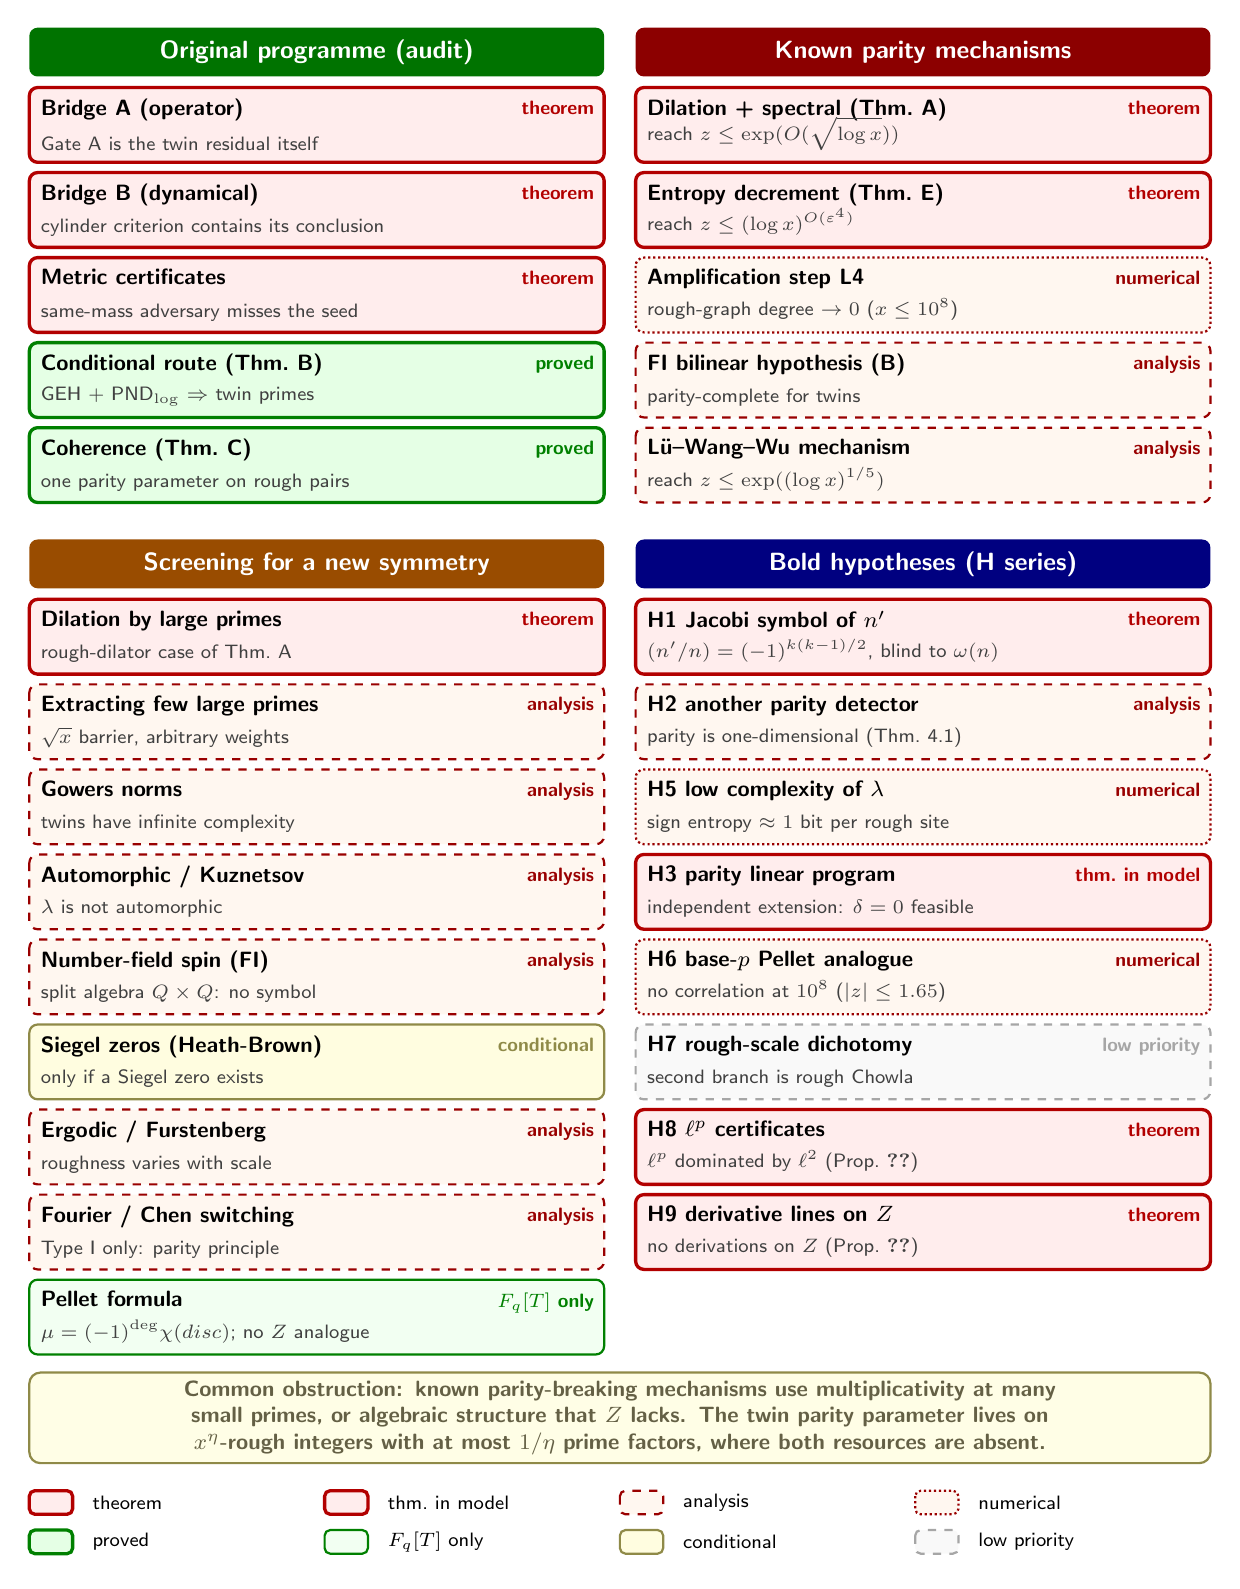
\begin{tikzpicture}[font=\sffamily]
\node[fill=green!45!black, text=white, minimum width=7.3cm, minimum height=0.62cm, inner xsep=0pt, outer sep=0pt, rounded corners=3pt, font=\small\bfseries\sffamily] at (3.650,0.450) {Original programme (audit)};
\draw[very thick, draw=red!70!black, fill=red!7, rounded corners=3pt] (0.000,0.000) rectangle (7.300,-0.950);
\node[anchor=north west, font=\footnotesize\bfseries\sffamily, inner sep=0pt] at (0.140,-0.140) {Bridge A (operator)};
\node[anchor=north east, font=\scriptsize\bfseries\sffamily, text=red!70!black, inner sep=0pt] at (7.180,-0.160) {theorem};
\node[anchor=south west, font=\scriptsize\sffamily, text=black!75, inner sep=0pt] at (0.140,-0.810) {Gate A is the twin residual itself};
\draw[very thick, draw=red!70!black, fill=red!7, rounded corners=3pt] (0.000,-1.080) rectangle (7.300,-2.030);
\node[anchor=north west, font=\footnotesize\bfseries\sffamily, inner sep=0pt] at (0.140,-1.220) {Bridge B (dynamical)};
\node[anchor=north east, font=\scriptsize\bfseries\sffamily, text=red!70!black, inner sep=0pt] at (7.180,-1.240) {theorem};
\node[anchor=south west, font=\scriptsize\sffamily, text=black!75, inner sep=0pt] at (0.140,-1.890) {cylinder criterion contains its conclusion};
\draw[very thick, draw=red!70!black, fill=red!7, rounded corners=3pt] (0.000,-2.160) rectangle (7.300,-3.110);
\node[anchor=north west, font=\footnotesize\bfseries\sffamily, inner sep=0pt] at (0.140,-2.300) {Metric certificates};
\node[anchor=north east, font=\scriptsize\bfseries\sffamily, text=red!70!black, inner sep=0pt] at (7.180,-2.320) {theorem};
\node[anchor=south west, font=\scriptsize\sffamily, text=black!75, inner sep=0pt] at (0.140,-2.970) {same-mass adversary misses the seed};
\draw[very thick, draw=green!50!black, fill=green!10, rounded corners=3pt] (0.000,-3.240) rectangle (7.300,-4.190);
\node[anchor=north west, font=\footnotesize\bfseries\sffamily, inner sep=0pt] at (0.140,-3.380) {Conditional route (Thm.~B)};
\node[anchor=north east, font=\scriptsize\bfseries\sffamily, text=green!50!black, inner sep=0pt] at (7.180,-3.400) {proved};
\node[anchor=south west, font=\scriptsize\sffamily, text=black!75, inner sep=0pt] at (0.140,-4.050) {GEH + PND$_{\log}$ $\Rightarrow$ twin primes};
\draw[very thick, draw=green!50!black, fill=green!10, rounded corners=3pt] (0.000,-4.320) rectangle (7.300,-5.270);
\node[anchor=north west, font=\footnotesize\bfseries\sffamily, inner sep=0pt] at (0.140,-4.460) {Coherence (Thm.~C)};
\node[anchor=north east, font=\scriptsize\bfseries\sffamily, text=green!50!black, inner sep=0pt] at (7.180,-4.480) {proved};
\node[anchor=south west, font=\scriptsize\sffamily, text=black!75, inner sep=0pt] at (0.140,-5.130) {one parity parameter on rough pairs};
\node[fill=red!55!black, text=white, minimum width=7.3cm, minimum height=0.62cm, inner xsep=0pt, outer sep=0pt, rounded corners=3pt, font=\small\bfseries\sffamily] at (11.350,0.450) {Known parity mechanisms};
\draw[very thick, draw=red!70!black, fill=red!7, rounded corners=3pt] (7.700,0.000) rectangle (15.000,-0.950);
\node[anchor=north west, font=\footnotesize\bfseries\sffamily, inner sep=0pt] at (7.840,-0.140) {Dilation + spectral (Thm.~A)};
\node[anchor=north east, font=\scriptsize\bfseries\sffamily, text=red!70!black, inner sep=0pt] at (14.880,-0.160) {theorem};
\node[anchor=south west, font=\scriptsize\sffamily, text=black!75, inner sep=0pt] at (7.840,-0.810) {reach $z\le\exp(O(\sqrt{\log x}))$};
\draw[very thick, draw=red!70!black, fill=red!7, rounded corners=3pt] (7.700,-1.080) rectangle (15.000,-2.030);
\node[anchor=north west, font=\footnotesize\bfseries\sffamily, inner sep=0pt] at (7.840,-1.220) {Entropy decrement (Thm.~E)};
\node[anchor=north east, font=\scriptsize\bfseries\sffamily, text=red!70!black, inner sep=0pt] at (14.880,-1.240) {theorem};
\node[anchor=south west, font=\scriptsize\sffamily, text=black!75, inner sep=0pt] at (7.840,-1.890) {reach $z\le(\log x)^{O(\varepsilon^4)}$};
\draw[thick, densely dotted, draw=red!60!black, fill=orange!6, rounded corners=3pt] (7.700,-2.160) rectangle (15.000,-3.110);
\node[anchor=north west, font=\footnotesize\bfseries\sffamily, inner sep=0pt] at (7.840,-2.300) {Amplification step L4};
\node[anchor=north east, font=\scriptsize\bfseries\sffamily, text=red!60!black, inner sep=0pt] at (14.880,-2.320) {numerical};
\node[anchor=south west, font=\scriptsize\sffamily, text=black!75, inner sep=0pt] at (7.840,-2.970) {rough-graph degree $\to0$ ($x\le10^8$)};
\draw[thick, dashed, draw=red!60!black, fill=orange!6, rounded corners=3pt] (7.700,-3.240) rectangle (15.000,-4.190);
\node[anchor=north west, font=\footnotesize\bfseries\sffamily, inner sep=0pt] at (7.840,-3.380) {FI bilinear hypothesis (B)};
\node[anchor=north east, font=\scriptsize\bfseries\sffamily, text=red!60!black, inner sep=0pt] at (14.880,-3.400) {analysis};
\node[anchor=south west, font=\scriptsize\sffamily, text=black!75, inner sep=0pt] at (7.840,-4.050) {parity-complete for twins};
\draw[thick, dashed, draw=red!60!black, fill=orange!6, rounded corners=3pt] (7.700,-4.320) rectangle (15.000,-5.270);
\node[anchor=north west, font=\footnotesize\bfseries\sffamily, inner sep=0pt] at (7.840,-4.460) {L\"u--Wang--Wu mechanism};
\node[anchor=north east, font=\scriptsize\bfseries\sffamily, text=red!60!black, inner sep=0pt] at (14.880,-4.480) {analysis};
\node[anchor=south west, font=\scriptsize\sffamily, text=black!75, inner sep=0pt] at (7.840,-5.130) {reach $z\le\exp((\log x)^{1/5})$};
\node[fill=orange!60!black, text=white, minimum width=7.3cm, minimum height=0.62cm, inner xsep=0pt, outer sep=0pt, rounded corners=3pt, font=\small\bfseries\sffamily] at (3.650,-6.050) {Screening for a new symmetry};
\draw[very thick, draw=red!70!black, fill=red!7, rounded corners=3pt] (0.000,-6.500) rectangle (7.300,-7.450);
\node[anchor=north west, font=\footnotesize\bfseries\sffamily, inner sep=0pt] at (0.140,-6.640) {Dilation by large primes};
\node[anchor=north east, font=\scriptsize\bfseries\sffamily, text=red!70!black, inner sep=0pt] at (7.180,-6.660) {theorem};
\node[anchor=south west, font=\scriptsize\sffamily, text=black!75, inner sep=0pt] at (0.140,-7.310) {rough-dilator case of Thm.~A};
\draw[thick, dashed, draw=red!60!black, fill=orange!6, rounded corners=3pt] (0.000,-7.580) rectangle (7.300,-8.530);
\node[anchor=north west, font=\footnotesize\bfseries\sffamily, inner sep=0pt] at (0.140,-7.720) {Extracting few large primes};
\node[anchor=north east, font=\scriptsize\bfseries\sffamily, text=red!60!black, inner sep=0pt] at (7.180,-7.740) {analysis};
\node[anchor=south west, font=\scriptsize\sffamily, text=black!75, inner sep=0pt] at (0.140,-8.390) {$\sqrt x$ barrier, arbitrary weights};
\draw[thick, dashed, draw=red!60!black, fill=orange!6, rounded corners=3pt] (0.000,-8.660) rectangle (7.300,-9.610);
\node[anchor=north west, font=\footnotesize\bfseries\sffamily, inner sep=0pt] at (0.140,-8.800) {Gowers norms};
\node[anchor=north east, font=\scriptsize\bfseries\sffamily, text=red!60!black, inner sep=0pt] at (7.180,-8.820) {analysis};
\node[anchor=south west, font=\scriptsize\sffamily, text=black!75, inner sep=0pt] at (0.140,-9.470) {twins have infinite complexity};
\draw[thick, dashed, draw=red!60!black, fill=orange!6, rounded corners=3pt] (0.000,-9.740) rectangle (7.300,-10.690);
\node[anchor=north west, font=\footnotesize\bfseries\sffamily, inner sep=0pt] at (0.140,-9.880) {Automorphic / Kuznetsov};
\node[anchor=north east, font=\scriptsize\bfseries\sffamily, text=red!60!black, inner sep=0pt] at (7.180,-9.900) {analysis};
\node[anchor=south west, font=\scriptsize\sffamily, text=black!75, inner sep=0pt] at (0.140,-10.550) {$\lambda$ is not automorphic};
\draw[thick, dashed, draw=red!60!black, fill=orange!6, rounded corners=3pt] (0.000,-10.820) rectangle (7.300,-11.770);
\node[anchor=north west, font=\footnotesize\bfseries\sffamily, inner sep=0pt] at (0.140,-10.960) {Number-field spin (FI)};
\node[anchor=north east, font=\scriptsize\bfseries\sffamily, text=red!60!black, inner sep=0pt] at (7.180,-10.980) {analysis};
\node[anchor=south west, font=\scriptsize\sffamily, text=black!75, inner sep=0pt] at (0.140,-11.630) {split algebra $\mathbb Q\times\mathbb Q$: no symbol};
\draw[thick, draw=yellow!50!black, fill=yellow!12, rounded corners=3pt] (0.000,-11.900) rectangle (7.300,-12.850);
\node[anchor=north west, font=\footnotesize\bfseries\sffamily, inner sep=0pt] at (0.140,-12.040) {Siegel zeros (Heath-Brown)};
\node[anchor=north east, font=\scriptsize\bfseries\sffamily, text=yellow!50!black, inner sep=0pt] at (7.180,-12.060) {conditional};
\node[anchor=south west, font=\scriptsize\sffamily, text=black!75, inner sep=0pt] at (0.140,-12.710) {only if a Siegel zero exists};
\draw[thick, dashed, draw=red!60!black, fill=orange!6, rounded corners=3pt] (0.000,-12.980) rectangle (7.300,-13.930);
\node[anchor=north west, font=\footnotesize\bfseries\sffamily, inner sep=0pt] at (0.140,-13.120) {Ergodic / Furstenberg};
\node[anchor=north east, font=\scriptsize\bfseries\sffamily, text=red!60!black, inner sep=0pt] at (7.180,-13.140) {analysis};
\node[anchor=south west, font=\scriptsize\sffamily, text=black!75, inner sep=0pt] at (0.140,-13.790) {roughness varies with scale};
\draw[thick, dashed, draw=red!60!black, fill=orange!6, rounded corners=3pt] (0.000,-14.060) rectangle (7.300,-15.010);
\node[anchor=north west, font=\footnotesize\bfseries\sffamily, inner sep=0pt] at (0.140,-14.200) {Fourier / Chen switching};
\node[anchor=north east, font=\scriptsize\bfseries\sffamily, text=red!60!black, inner sep=0pt] at (7.180,-14.220) {analysis};
\node[anchor=south west, font=\scriptsize\sffamily, text=black!75, inner sep=0pt] at (0.140,-14.870) {Type I only: parity principle};
\draw[thick, draw=green!50!black, fill=green!5, rounded corners=3pt] (0.000,-15.140) rectangle (7.300,-16.090);
\node[anchor=north west, font=\footnotesize\bfseries\sffamily, inner sep=0pt] at (0.140,-15.280) {Pellet formula};
\node[anchor=north east, font=\scriptsize\bfseries\sffamily, text=green!50!black, inner sep=0pt] at (7.180,-15.300) {$\mathbb F_q[T]$ only};
\node[anchor=south west, font=\scriptsize\sffamily, text=black!75, inner sep=0pt] at (0.140,-15.950) {$\mu=(-1)^{\deg}\chi(\operatorname{disc})$; no $\mathbb Z$ analogue};
\node[fill=blue!50!black, text=white, minimum width=7.3cm, minimum height=0.62cm, inner xsep=0pt, outer sep=0pt, rounded corners=3pt, font=\small\bfseries\sffamily] at (11.350,-6.050) {Bold hypotheses (H series)};
\draw[very thick, draw=red!70!black, fill=red!7, rounded corners=3pt] (7.700,-6.500) rectangle (15.000,-7.450);
\node[anchor=north west, font=\footnotesize\bfseries\sffamily, inner sep=0pt] at (7.840,-6.640) {H1 Jacobi symbol of $n'$};
\node[anchor=north east, font=\scriptsize\bfseries\sffamily, text=red!70!black, inner sep=0pt] at (14.880,-6.660) {theorem};
\node[anchor=south west, font=\scriptsize\sffamily, text=black!75, inner sep=0pt] at (7.840,-7.310) {$(n'/n)=(-1)^{k(k-1)/2}$, blind to $\omega(n)$};
\draw[thick, dashed, draw=red!60!black, fill=orange!6, rounded corners=3pt] (7.700,-7.580) rectangle (15.000,-8.530);
\node[anchor=north west, font=\footnotesize\bfseries\sffamily, inner sep=0pt] at (7.840,-7.720) {H2 another parity detector};
\node[anchor=north east, font=\scriptsize\bfseries\sffamily, text=red!60!black, inner sep=0pt] at (14.880,-7.740) {analysis};
\node[anchor=south west, font=\scriptsize\sffamily, text=black!75, inner sep=0pt] at (7.840,-8.390) {parity is one-dimensional (Thm.~4.1)};
\draw[thick, densely dotted, draw=red!60!black, fill=orange!6, rounded corners=3pt] (7.700,-8.660) rectangle (15.000,-9.610);
\node[anchor=north west, font=\footnotesize\bfseries\sffamily, inner sep=0pt] at (7.840,-8.800) {H5 low complexity of $\lambda$};
\node[anchor=north east, font=\scriptsize\bfseries\sffamily, text=red!60!black, inner sep=0pt] at (14.880,-8.820) {numerical};
\node[anchor=south west, font=\scriptsize\sffamily, text=black!75, inner sep=0pt] at (7.840,-9.470) {sign entropy $\approx1$ bit per rough site};
\draw[very thick, draw=red!70!black, fill=red!7, rounded corners=3pt] (7.700,-9.740) rectangle (15.000,-10.690);
\node[anchor=north west, font=\footnotesize\bfseries\sffamily, inner sep=0pt] at (7.840,-9.880) {H3 parity linear program};
\node[anchor=north east, font=\scriptsize\bfseries\sffamily, text=red!70!black, inner sep=0pt] at (14.880,-9.900) {thm.\ in model};
\node[anchor=south west, font=\scriptsize\sffamily, text=black!75, inner sep=0pt] at (7.840,-10.550) {independent extension: $\delta=0$ feasible};
\draw[thick, densely dotted, draw=red!60!black, fill=orange!6, rounded corners=3pt] (7.700,-10.820) rectangle (15.000,-11.770);
\node[anchor=north west, font=\footnotesize\bfseries\sffamily, inner sep=0pt] at (7.840,-10.960) {H6 base-$p$ Pellet analogue};
\node[anchor=north east, font=\scriptsize\bfseries\sffamily, text=red!60!black, inner sep=0pt] at (14.880,-10.980) {numerical};
\node[anchor=south west, font=\scriptsize\sffamily, text=black!75, inner sep=0pt] at (7.840,-11.630) {no correlation at $10^8$ ($|z|\le1.65$)};
\draw[thick, dashed, draw=gray!70, fill=gray!5, rounded corners=3pt] (7.700,-11.900) rectangle (15.000,-12.850);
\node[anchor=north west, font=\footnotesize\bfseries\sffamily, inner sep=0pt] at (7.840,-12.040) {H7 rough-scale dichotomy};
\node[anchor=north east, font=\scriptsize\bfseries\sffamily, text=gray!70, inner sep=0pt] at (14.880,-12.060) {low priority};
\node[anchor=south west, font=\scriptsize\sffamily, text=black!75, inner sep=0pt] at (7.840,-12.710) {second branch is rough Chowla};
\draw[very thick, draw=red!70!black, fill=red!7, rounded corners=3pt] (7.700,-12.980) rectangle (15.000,-13.930);
\node[anchor=north west, font=\footnotesize\bfseries\sffamily, inner sep=0pt] at (7.840,-13.120) {H8 $\ell^p$ certificates};
\node[anchor=north east, font=\scriptsize\bfseries\sffamily, text=red!70!black, inner sep=0pt] at (14.880,-13.140) {theorem};
\node[anchor=south west, font=\scriptsize\sffamily, text=black!75, inner sep=0pt] at (7.840,-13.790) {$\ell^p$ dominated by $\ell^2$ (Prop.~\ref{prop:L})};
\draw[very thick, draw=red!70!black, fill=red!7, rounded corners=3pt] (7.700,-14.060) rectangle (15.000,-15.010);
\node[anchor=north west, font=\footnotesize\bfseries\sffamily, inner sep=0pt] at (7.840,-14.200) {H9 derivative lines on $\mathbb Z$};
\node[anchor=north east, font=\scriptsize\bfseries\sffamily, text=red!70!black, inner sep=0pt] at (14.880,-14.220) {theorem};
\node[anchor=south west, font=\scriptsize\sffamily, text=black!75, inner sep=0pt] at (7.840,-14.870) {no derivations on $\mathbb Z$ (Prop.~\ref{prop:noderiv})};
\draw[thick, draw=yellow!50!black, fill=yellow!10, rounded corners=4pt] (0,-16.320) rectangle (15.000,-17.470);
\node[align=center, text width=14.60cm, font=\footnotesize\bfseries\sffamily, text=yellow!30!black] at (7.500,-16.895) {Common obstruction: known parity-breaking mechanisms use multiplicativity at many small primes, or algebraic structure that $\mathbb Z$ lacks. The twin parity parameter lives on $x^\eta$-rough integers with at most $1/\eta$ prime factors, where both resources are absent.};
\draw[very thick, draw=red!70!black, fill=red!7, rounded corners=2pt] (0.000,-17.820) rectangle (0.550,-18.120);
\node[anchor=west, font=\scriptsize\sffamily] at (0.680,-17.970) {theorem};
\draw[very thick, draw=red!70!black, fill=red!7, rounded corners=2pt] (3.750,-17.820) rectangle (4.300,-18.120);
\node[anchor=west, font=\scriptsize\sffamily] at (4.430,-17.970) {thm.\ in model};
\draw[thick, dashed, draw=red!60!black, fill=orange!6, rounded corners=2pt] (7.500,-17.820) rectangle (8.050,-18.120);
\node[anchor=west, font=\scriptsize\sffamily] at (8.180,-17.970) {analysis};
\draw[thick, densely dotted, draw=red!60!black, fill=orange!6, rounded corners=2pt] (11.250,-17.820) rectangle (11.800,-18.120);
\node[anchor=west, font=\scriptsize\sffamily] at (11.930,-17.970) {numerical};
\draw[very thick, draw=green!50!black, fill=green!10, rounded corners=2pt] (0.000,-18.320) rectangle (0.550,-18.620);
\node[anchor=west, font=\scriptsize\sffamily] at (0.680,-18.470) {proved};
\draw[thick, draw=green!50!black, fill=green!5, rounded corners=2pt] (3.750,-18.320) rectangle (4.300,-18.620);
\node[anchor=west, font=\scriptsize\sffamily] at (4.430,-18.470) {$\mathbb F_q[T]$ only};
\draw[thick, draw=yellow!50!black, fill=yellow!12, rounded corners=2pt] (7.500,-18.320) rectangle (8.050,-18.620);
\node[anchor=west, font=\scriptsize\sffamily] at (8.180,-18.470) {conditional};
\draw[thick, dashed, draw=gray!70, fill=gray!5, rounded corners=2pt] (11.250,-18.320) rectangle (11.800,-18.620);
\node[anchor=west, font=\scriptsize\sffamily] at (11.930,-18.470) {low priority};
\end{tikzpicture}}
\caption{Map of every route explored in this project, with its status. ``Theorem'' means a complete proof in this paper or in the separate audit of the original programme (first column); ``thm.\ in model'' means an explicit construction that is rigorous within the stated model; ``analysis'' and ``numerical'' are judgements about specific arguments or data, not theorems. All entries were obtained with AI assistance and have not yet been checked by a specialist (Appendix~\ref{app:ai}).}
\label{fig:exploration}
\end{figure}


\paragraph{The Friedlander--Iwaniec bilinear hypothesis.} In the asymptotic sieve for primes \cite{FI98}, parity is broken by a bilinear hypothesis (B). For the twin sequence $a_k=\mathbf 1_{\mathbb P}(k+2)$ it reads
\[
\sum_m\Bigl|\sum_{N<n\le2N}\gamma(n,C)\mu(n)\mathbf 1_{\mathbb P}(mn+2)\Bigr|=o\Bigl(\frac{x}{\log x}\Bigr)
\]
for every $N$ in a range that always contains $N\approx\sqrt x$, with arbitrary coefficients on $m$ because of the absolute values. We tried three ways of reducing (B) to known estimates; each ends in an obstruction:
\begin{itemize}
\item a Heath-Brown decomposition of $\Lambda(mn+2)$ leaves a determinant sum over $mn-de=-2$ with Möbius-type coefficients on both sides, which is two-point Chowla on a determinant variety;
\item extracting small primes from the unshifted variable $n$, in the manner of \cite{LWW26}, removes $\mu$ but squares the prime side into a binary prime correlation, with coefficients larger than the range of the variable;
\item Cauchy--Schwarz in $m$ returns the $L^2$ form of (B) itself.
\end{itemize}
Beyond $\sqrt x$, distribution results with arbitrary coefficients are not known. We call (B) \emph{parity-complete} for twins: this is an analysis of known techniques, not an impossibility statement.

\paragraph{Screening for a new symmetry.} We tested nine classes of mechanisms against three criteria: (i) they must act on $x^\eta$-rough integers without extracting small primes; (ii) they must be parity-sensitive; (iii) they must not be blocked by a known obstruction. Only Pellet's formula $\mu(f)=(-1)^{\deg f}\chi(\operatorname{disc}f)$ over $\mathbb F_q[T]$ passes, and it is the mechanism behind the function-field twin prime theorem of Sawin and Shusterman \cite{SS22}. We verified it for all squarefree monic polynomials over $\mathbb F_3$ (degree $\le7$) and $\mathbb F_5$ (degree $\le5$), including those whose smallest irreducible factor has large degree. The reason it has no integer analogue is that, for fixed degree, $\mu$ on $\mathbb F_q[T]$ is a quadratic character of a polynomial in the coefficients, which Weil--Deligne estimates can control. No comparable structure is known for $\lambda$ on $\mathbb Z$.

\paragraph{The H series.} Table~\ref{tab:hledger} lists the bold hypotheses and their fate.

\begin{table}[H]
\centering
\small
\begin{tabular}{p{3.4cm}p{1.6cm}p{7.4cm}}
\toprule
hypothesis & status & reason\\
\midrule
H1: the Jacobi symbol of the arithmetic derivative $n'=\sum_{p\mid n}n/p$ detects $(-1)^{\omega(n)}$ & false (proof) & For odd squarefree $n$, quadratic reciprocity gives $(n'/n)=(-1)^{k(k-1)/2}$ with $k=\#\{p\mid n:p\equiv3\bmod4\}$, so the symbol is blind to $\omega(n)$. Checked for all $81{,}053$ cases $n\le2\cdot10^5$; agreement with $\lambda$ is $0.4935$.\\
H2: a different parity detector is easier to control & false (analysis) & By Theorem~\ref{thm:onesided}, every detector separating primes from $P_2$ is governed by the same parameter $\delta$.\\
H3: positivity across many patterns forces $\delta_{\rm twin}>0$ & false (model) & A linear program with patterns of $3$ and $4$ shifts, up to $966$ variables, gives $\delta_{\rm twin}\in[0,2]$ in every case. Explicit witness: the extreme counterfeit on $(n,n+2)$, extended independently to all other entries.\\
H5: $\lambda$ has low complexity on rough integers & false (numerical) & The sign entropy is about $1$ bit per rough site up to $x=10^8$.\\
H6: $\lambda(n)$ correlates with the function-field Möbius of the base-$p$ digit polynomial of $n$ & false (numerical) & With $p=463$ ($d=2$) and $p=97$ ($d=3$), about $10^8$ integers each, all twelve correlations (for $\lambda$, $\mu$ and rough $\lambda$) are within noise, $|z|\le1.65$, so $|\mathrm{corr}|\lesssim3\cdot10^{-4}$.\\
H7: a Heath-Brown type dichotomy at rough scale & open (low priority) & Its second branch is the Chowla conjecture on rough integers.\\
H9: $\lambda$ is a Dirichlet character on a positive-density family of integer ``lines'', as $\mu$ is in $\mathbb F_q[T]$ & false (proof and numerical) & There are no derivations on $\mathbb Z$, local substitutes give periodic functions, and permutation-sign discriminants are Jacobi symbols (Proposition~\ref{prop:noderiv}). Line-dependent large-conductor Jacobi symbols: twelve tests at $x=10^8$ within noise, planted control $z\approx800$ (Remark~\ref{rem:H9}).\\
H10--H16: techniques from 2026 AI-generated papers (bounded independence, prime-slot Type~II, zero-free regions, exclusion of Siegel zeros, weighted vertices, Hardy--Littlewood--Chowla transfer, dictionary search) give parity on rough pairs & false (analysis and numerical) & Each takes its sign from small primes or gives no bound beyond $0\le\delta\le2$; numerical cards null at $x=10^8$ with controls at $z\approx565$--$811$. Weighted vertices led to the improved Proposition~\ref{prop:T}.\\
H17--H23: structure for $\sum a_mb_n\lambda(mn+2)$ (dispersion, low rank, norm forms, entropy decrement in a prime variable, small characters, residue forcing, Mellin) & false (analysis and numerical) & Remark~\ref{rem:cards}; the Mellin test led to the absolute-value barrier of Remark~\ref{rem:mellin}.\\
H8: $\ell^p$ or weighted $\ell^2$ certificates pass the $t$-ceiling of Proposition~\ref{prop:T} & false ($\ell^p$: proof); weighted: numerical & $\ell^p$ certificates are dominated by $\ell^2$ (Proposition~\ref{prop:L}). Weights $|g_t|^\beta$ improve the resolution only by constant factors at $x=10^7$, with no detectable change of exponent.\\
\bottomrule
\end{tabular}
\caption{The hypothesis ledger.}
\label{tab:hledger}
\end{table}

\noindent Two lessons from the ledger are worth recording.
\begin{itemize}
\item In H3, the base mass in the one-sided constraints must be the \emph{actual} mass of the sub-pattern, which is itself a variable. A first hand computation that used the model mass instead appeared to force $\delta\approx1$; that was a false positive.
\item In H6, integer carries make multiplication incompatible with digit polynomials, which is why $\lambda$ and the digit-polynomial Möbius function are unrelated.
\end{itemize}
Every reason recorded above points to the obstruction stated in Remark~\ref{rem:common}.

\subsection{Limitations}
All proofs were drafted and checked within the same AI-assisted process. None has yet been independently checked by a human specialist, and errors of the kind listed above may remain. The following points are the most delicate:
\begin{itemize}
\item the uniform upper bound (U) in Theorem~\ref{thm:onesided};
\item the treatment of boundary boxes in Lemma~\ref{lem:geh-box};
\item conditions (A3)--(A4) of Definition~\ref{def:cert}, in particular whether the rarer exceptional sets of \cite{HR21,Pil23} meet at most half of $\mathcal K$;
\item in Proposition~\ref{prop:T}, the uniformity in $t$ of the Selberg--Delange and Nair--Tenenbaum inputs, which are used as black boxes;
\item in Proposition~\ref{prop:Q}, the axioms for the difference sequence $b$, and the size of $\varepsilon(x)$, which we have not quantified;
\item in Section~\ref{sec:locate}, the census of Table~\ref{tab:census} is not claimed to be exhaustive, Remark~\ref{rem:MRT} is an analysis of one proof, and Proposition~\ref{prop:absbarrier} is proved for the Bohr mean and, by Corollary~\ref{cor:absbarrierT}, for windows $T\gg x^4$, but not for the windows $T\asymp x$ used in practice, and only for prime supports, with a very small constant;
\item Remark~\ref{rem:conjA} comes from a separate AI session and is conditional on Conjecture~A, which is supported only numerically;
\item the 2026 AI-generated preprints cited as \cite{OpenAI26} have not been refereed, and we did not check their proofs;
\item in Proposition~\ref{prop:disjunction}, we rely on the published construction of the weights in \cite{Polymath8b} and have not re-derived Theorems~3.14 and~3.15 there.
\end{itemize}
Bombieri's original paper, Chapter~16 of \cite{FI10}, and \cite{MV17} were not read in full. We would be grateful for corrections.
